%% Paper E -- Computacion y Sistemas (CyS) template: cys.cls, cys.bst.
%% SOURCE FILE. paper_e.tex is generated from this file by scripts/build_paper_e.py, which
%% replaces every double-angle placeholder with a value read from outputs/analysis/paper_e/.
%% Do not type a result by hand.
%%
%% Review is blind: the default build omits author identity and the repository address.
%% The full build defines \fullversion before this file is read.
\documentclass{cys}

% The class asks for Helvetica (the journal's Arial). Under XeTeX (Tectonic) that needs fontspec.
\usepackage{iftex}
\ifPDFTeX
  \usepackage[utf8]{inputenc}
\else
  \usepackage{fontspec}
  \setmainfont{texgyreheros}[Extension=.otf,UprightFont=*-regular,BoldFont=*-bold,
    ItalicFont=*-italic,BoldItalicFont=*-bolditalic]
  \setsansfont{texgyreheros}[Extension=.otf,UprightFont=*-regular,BoldFont=*-bold,
    ItalicFont=*-italic,BoldItalicFont=*-bolditalic]
\fi
\usepackage[english]{babel}
\usepackage{graphicx}
\usepackage{amsmath}
\usepackage{url}
\usepackage{cite}

\addto\captionsenglish{%
  \renewcommand{\figurename}{Fig.}%
  \renewcommand{\abstractname}{Abstract.}%
}
\setlength{\emergencystretch}{3em}
%% Paper E layout constants. Kept out of paper_e.tex because that file is under
%% [coverage] in pub/claim_registry.toml, where every decimal must be a registered result.
\newcommand{\tablestretch}{1.1}
\newlength{\tightcolsep}\setlength{\tightcolsep}{2.2pt}
\newlength{\mediumcolsep}\setlength{\mediumcolsep}{3pt}

%% Code and data archive (full version only). Set after the GitHub release is archived by
%% Zenodo; see README.md, "Release and archive".
\newcommand{\papererelease}{paper-e-cys-2026-10-04-r2}
\newcommand{\paperearchive}{\url{https://doi.org/10.5281/zenodo.23142429}}


\newif\iffull
\ifdefined\fullversion \fulltrue \else \fullfalse \fi

\title{Do Explainers Agree on Which Features Matter? \\ Instance-Level Agreement between SHAP and LIME \\ on Three Tabular Datasets}

\iffull
\author{Jonathan Herrera-V\'asquez$^{*}$}
\affil{
Universidad Americana de Europa (UNADE), Department of Computer Science, Canc\'un, \authorcr
Mexico
\authorcr \authorcr
jonnabio@gmail.com
\authorcr \authorcr
}
\else
\author{Author information omitted for blind review}
\affil{\authorcr}
\fi

\begin{document}

\maketitle

\renewcommand{\tablename}{Table}

\begin{abstract}
Post-hoc explainers are often used as if they were interchangeable, yet two explainers may
name different features for the same prediction. This study measures how much SHAP and LIME
agree at the level of the single instance. Both methods explained the same instances of
the same models on three tabular datasets (Adult, German Credit and Breast Cancer
Wisconsin), giving <<n|paired>> paired explanations in <<n|primary_runs>> runs. The
analysis plan was registered before any agreement statistic was computed; runs, not
instances, are the unit of summary, and intervals resample random seeds. The mean overlap
of the five most important features (Jaccard index) was <<agree|exp2_adult|all|top5_jaccard|est>>
on Adult, <<agree|german_credit|all|top5_jaccard|est>> on German Credit and
<<agree|breast_cancer|all|top5_jaccard|est>> on Breast Cancer, well above the overlap of
random feature sets but far from identity, and the ordering of the features agreed
weakly on two of the three datasets. Agreement depended on the model family and did not
depend on the number of explained instances. It was not consistently lower for
misclassified instances. Disagreement was larger where the local fidelity of LIME was
lower. A post hoc analysis shows that the agreement of signs between the two methods is
driven by the predicted class, because LIME without discretisation returns local slopes
while SHAP returns signed contributions; sign agreement between them should not be read
as a measure of disagreement.
\end{abstract}

\begin{keywords}
Explainable artificial intelligence, post-hoc explanations, disagreement problem, feature attribution, SHAP, LIME.
\end{keywords}

\section{Introduction}
\label{sec:introduction}

Post-hoc explanation methods describe a prediction of a trained model in terms of its input
features. SHAP \cite{lundberg2017unified} and LIME \cite{ribeiro2016why} are the most used
for tabular data: each returns, for one instance, a signed weight per feature. In practice
the two are treated as alternatives, and the choice between them is made on cost or habit.
That practice assumes that the explanation a user sees does not depend much on the method.

The assumption has been questioned. Krishna et al. \cite{krishna2024disagreement} named
the \emph{disagreement problem}: explanation methods often identify different top
features for the same prediction, and practitioners have no principled way to resolve the
conflict. Similar observations were made for text models \cite{neely2021order} and for
defect prediction \cite{roy2022why}. If the features shown to a user change with the
explainer, an explanation is a property of the pair (model, explainer), not of the model
alone, and conclusions drawn from it need the same caution
\cite{rudin2019stop,doshivelez2017rigorous}.

Most evidence on disagreement comes from a small number of models per dataset and treats
the explained instances as independent observations. Two points remain open for tabular
classifiers. The first is how much agreement varies with the model family, the dataset
and the number of explained instances when the same instances are explained by both
methods. The second is whether disagreement is related to two properties that
practitioners care about: whether the prediction is correct, and how good each
explanation is by the usual quality measures.

This study addresses both points with instance-paired explanations from an existing
benchmark cohort and a new, instance-aligned cohort produced for this purpose. The
research questions are:

\begin{itemize}
\item \textbf{RQ1.} For the same instance and model, how much do SHAP and LIME agree on
the most influential features and on their order?
\item \textbf{RQ2.} How does this agreement vary with the model family, the sampling
intensity and the dataset?
\item \textbf{RQ3.} Is agreement different for correctly classified and misclassified
instances?
\item \textbf{RQ4.} Is disagreement on an instance associated with the fidelity or the
stability of either explanation?
\end{itemize}

A secondary, descriptive question is how the features used by two explainers of a
different kind, Anchors \cite{ribeiro2018anchors} and DiCE \cite{mothilal2020dice},
overlap with those of SHAP and LIME.

The contributions are: (i) estimates of SHAP--LIME agreement on <<n|paired>> paired
explanations across five model families and three datasets, with the run as the unit of
summary and intervals clustered by random seed; (ii) evidence that agreement depends on
the model family and the dataset, not on the number of explained instances, and is not
consistently related to prediction correctness; (iii) an association between
disagreement and the local fidelity of LIME; and (iv) a methodological finding: the sign
agreement between SHAP and LIME without discretisation is determined mostly by the
predicted class, because the two methods return different quantities.

\section{Related Work}
\label{sec:related}

\textbf{Disagreement between explainers.} Krishna et al. \cite{krishna2024disagreement}
formalised disagreement with measures of feature agreement, rank agreement, sign
agreement and rank correlation over the top-$k$ features, and reported frequent
disagreement across datasets and models, together with interviews showing that
practitioners resolve it with ad hoc rules. Neely et al. \cite{neely2021order} found low
rank correlation between attribution methods for text classifiers and argued that
agreement should not be used to validate a method. Roy et al. \cite{roy2022why}
reported disagreement between LIME and SHAP for defect prediction models, on the
features and on their sign.

\textbf{Why methods differ.} Han et al. \cite{han2022which} showed that several
attribution methods are local function approximations of the model that differ in the
neighbourhood and the loss they use, so that no method is best for every neighbourhood.
Garreau and von Luxburg \cite{garreau2020explaining} analysed LIME for tabular data and
showed that, for a linear model, its coefficients are proportional to the gradient of
the model. SHAP values, in contrast, distribute the difference between the prediction and
an expected prediction among the features \cite{lundberg2017unified,lundberg2020local}.
This difference of meaning matters for the sign analysis in
Section~\ref{sec:results:sign}.

\textbf{Reliability of explanations.} Explanations can change under small perturbations
of the input \cite{alvarezmelis2018robustness} and can be manipulated
\cite{slack2020fooling}. Stability and fidelity are therefore common quality criteria.
This study relates them to disagreement at the level of the instance, which, to our
knowledge, earlier work on tabular data has not reported with a clustered design.

\section{Materials and Methods}
\label{sec:methods}

\subsection{Datasets, Models and Runs}

Three public binary classification datasets were used: Adult \cite{becker1996adult}
(108 encoded features), German Credit \cite{hofmann1994statlog} (61 encoded features) and
Breast Cancer Wisconsin, diagnostic \cite{wolberg1993breast} (30 numeric features).
Numeric features were standardised and categorical features were one-hot encoded; each
encoded column is one feature in every analysis.

On Adult, five model families were explained: logistic regression (LR), a support
vector machine with probability outputs (SVM), a multilayer perceptron (MLP), a random
forest (RF) \cite{breiman2001random} and gradient boosting (XGB) \cite{chen2016xgboost}.
Each explainer was run with five random seeds and three sampling intensities
($n = 50$, $100$ and $200$ test instances per quadrant of the confusion matrix), so that
correct and incorrect predictions are both represented. On German Credit and Breast
Cancer, RF and XGB models were trained with three seeds each and explained with one
intensity (up to 100 instances per quadrant).

\iffull
The Adult runs and the SHAP and Anchors runs of the other two datasets belong to a
benchmark cohort described in \cite{herrera2026framework}. That work compares explainers
by quality measures; no result of it is repeated here.
\else
The Adult runs and the SHAP and Anchors runs of the other two datasets belong to a
benchmark cohort described in an earlier publication (reference withheld for blind
review). That work compares explainers by quality measures; no result of it is repeated
here.
\fi
A companion manuscript under review studies explanation quality on correct and incorrect
predictions with the same cohort; it does not study agreement between explainers.

The earlier LIME runs on German Credit and Breast Cancer explained a different sample of
instances and stored only averages. \emph{A new LIME cohort was therefore produced for
this study}: for each dataset, model and seed, LIME explained exactly the instances
stored in the corresponding SHAP run. The model binaries were regenerated from the
training recipe in the repository, and the run was allowed only after the regenerated
model reproduced the stored training metrics, the feature order and the stored label and
prediction of every target instance.

\subsection{Explainers}
\label{sec:methods:explainers}

\textbf{SHAP.} TreeSHAP \cite{lundberg2020local} was used for RF and XGB, and KernelSHAP
\cite{lundberg2017unified} with 50 background instances for LR, SVM and MLP. The stored
value of a feature is its signed contribution to the output for class~1, relative to
the expected output on the background data.

\textbf{LIME.} The tabular explainer \cite{ribeiro2016why} was used with 1000 perturbed
samples, kernel width 3, ten selected features and \emph{without discretisation of
continuous features}. With this setting, the stored value of a feature is the
coefficient of the local weighted linear model for class~1, that is, a local slope.

\textbf{Anchors and DiCE} (Adult, secondary analysis). Anchors
\cite{ribeiro2018anchors} returns a rule; its feature set is the set of features in the
rule. DiCE \cite{mothilal2020dice} returns counterfactual instances; its feature set is
the set of features whose value changes. Neither is a signed attribution, so only
feature sets are compared.

For each instance, a run stores the ten features with the largest absolute value, in
that order. All measures below use these stored lists.

\subsection{Agreement Measures}

Let $S_k$ and $L_k$ be the sets of the $k$ features with the largest absolute SHAP and
LIME values for one instance. The primary measure is the top-5 Jaccard overlap
\cite{jaccard1912distribution}:
\begin{equation}
J_5 = \frac{|S_5 \cap L_5|}{|S_5 \cup L_5|}.
\label{eq:jaccard}
\end{equation}
Three shared features out of five give $J_5 = 3/7$, and four give $J_5 = 4/6$. The top-10 overlap $J_{10}$ is a sensitivity measure.

Rank concordance is Kendall's $\tau_b$ \cite{kendall1945treatment} computed on the union
of the two top-10 lists; a feature absent from a list receives rank 11, and ties use
midranks.

Sign agreement is the fraction of the features in $S_5 \cap L_5$, with both values
different from zero, whose SHAP and LIME values have the same sign.

As a reference, not as a threshold, the expected value of $J_k$ for two independent
random sets of $k$ features out of $p$ was computed exactly from the hypergeometric
distribution. For $k = 5$ it is <<chance|exp2_adult|5>> on Adult,
<<chance|german_credit|5>> on German Credit and <<chance|breast_cancer|5>> on Breast
Cancer.

\subsection{Pairing and Quality Control}

Explanations were paired by dataset, model, seed, intensity and instance identifier.
Only instances with a valid explanation from both methods and the same stored label and
prediction entered the analysis. The source runs contained <<n|invalid_rows>> records
with an error and no explanation, mostly KernelSHAP on the SVM; these were excluded,
and one SVM block had no usable SHAP run. Of the <<n|blocks>> blocks, <<n|exact_blocks>>
had identical sets of valid instances for the two methods; in the others the
intersection was used, which left <<n|unpaired>> valid records unpaired. No paired
record had a different label or prediction in the two runs. The result is <<n|paired>>
paired explanations in <<n|primary_runs>> runs: <<n|inst_exp2_adult>> on Adult
(<<n|runs_exp2_adult>> runs), <<n|inst_german_credit>> on German Credit and
<<n|inst_breast_cancer>> on Breast Cancer (six runs each). Kendall's $\tau_b$ was
undefined for <<n|tau_undefined>> pairs and sign agreement for <<n|sign_undefined>> pairs
without a shared non-zero feature.

\subsection{Statistical Summary}

The same test instances recur across models, seeds and intensities, so instances are not
independent replicates. Each measure was first averaged within a run (dataset, model,
seed, intensity). The point estimate of a group is the mean of its run means. The 95\%
interval is a percentile bootstrap with 2000 resamples in which random seeds, not
instances, are resampled with replacement, and all runs of a sampled seed are kept
together \cite{efron1993introduction,cameron2015practitioner}. There are five seeds on
Adult and three on the other datasets, so the intervals describe variation between seeds
and are not precise.

For RQ3, the difference between the mean $J_5$ of misclassified and of correctly
classified instances was computed within each run that had at least ten instances in
each group, averaged over intensities for each model and seed, and summarised by model.
For RQ4, the Spearman correlation between disagreement ($1 - J_5$) and each of four
quality values of the instance (fidelity and stability of the SHAP and of the LIME
explanation) was computed within each run and averaged by seed. Fidelity is the
coefficient of determination between the model output and its reconstruction from the
explanation weights on a neighbourhood of the instance; stability is the mean cosine
similarity between explanations of slightly perturbed copies of the instance. Both were
stored with each explanation when the runs were made.

No hypothesis test was planned and no $p$-value is reported. The estimates for RQ2 to RQ4
are exploratory.

\subsection{Registration and Deviations}

The analysis plan, with the measures, the unit of analysis, the exclusion rules and the
bootstrap settings, was committed to the repository before any agreement statistic was
computed and before the new LIME cohort was run. Two refinements made before the
analysis are recorded in the plan. One analysis is \emph{post hoc}: after the planned
sign agreement was inspected, it was broken down by predicted class and the constancy of
the sign of each feature was measured (Section~\ref{sec:results:sign}). It is reported
as such.

\section{Results}
\label{sec:results}

\subsection{Agreement on the Top Features (RQ1)}

Table~\ref{tab:agreement} and Fig.~\ref{fig:overlap} give the agreement estimates. On
Adult, the mean top-5 overlap was <<agree|exp2_adult|all|top5_jaccard|est>> (95\%
interval <<agree|exp2_adult|all|top5_jaccard|lo>> to
<<agree|exp2_adult|all|top5_jaccard|hi>>); on German Credit it was
<<agree|german_credit|all|top5_jaccard|est>> (<<agree|german_credit|all|top5_jaccard|lo>>
to <<agree|german_credit|all|top5_jaccard|hi>>). Both are below the value for three
shared features out of five. On Breast Cancer the overlap was
<<agree|breast_cancer|all|top5_jaccard|est>> (<<agree|breast_cancer|all|top5_jaccard|lo>>
to <<agree|breast_cancer|all|top5_jaccard|hi>>), above the value for four shared
features. In all three datasets the overlap was several times the expected overlap of
random sets.

The order of the features agreed less than their identity. Kendall's $\tau_b$ was
<<agree|exp2_adult|all|kendall_tau_b|est>> on Adult and
<<agree|german_credit|all|kendall_tau_b|est>> on German Credit, and
<<agree|breast_cancer|all|kendall_tau_b|est>> on Breast Cancer. Extending the lists to
ten features raised the overlap on Adult and German Credit
(<<agree|exp2_adult|all|top10_jaccard|est>> and
<<agree|german_credit|all|top10_jaccard|est>>) and lowered it slightly on Breast Cancer
(<<agree|breast_cancer|all|top10_jaccard|est>>).

\begin{table*}[t]
\renewcommand{\arraystretch}{\tablestretch}
\centering
\caption{Agreement between SHAP and LIME: mean of run means and seed-clustered 95\% interval. Adult rows pool the three sampling intensities}
\label{tab:agreement}
\small
\begin{tabular}{llrrlll}
\hline
Dataset & Model & Runs & Pairs & Top-5 Jaccard & Top-10 Jaccard & Kendall $\tau_b$ \\
\hline
% GENERATED by scripts/build_paper_e.py -- do not edit
Adult & LR & 15 & 7,000 & 0.485 [0.464, 0.505] & 0.261 & 0.617 [0.584, 0.640] & 0.263 [0.221, 0.304] \\
 & SVM & 14 & 2,064 & 0.395 [0.388, 0.404] & 0.206 & 0.516 [0.489, 0.539] & 0.171 [0.148, 0.187] \\
 & MLP & 15 & 7,000 & 0.335 [0.326, 0.341] & 0.128 & 0.441 [0.435, 0.448] & 0.043 [0.029, 0.054] \\
 & RF & 15 & 6,603 & 0.389 [0.360, 0.415] & 0.199 & 0.560 [0.530, 0.590] & 0.129 [0.090, 0.168] \\
 & XGB & 15 & 7,000 & 0.363 [0.328, 0.399] & 0.219 & 0.404 [0.384, 0.422] & 0.028 [$-$0.020, 0.071] \\
 & All & 74 & 29,667 & 0.393 [0.377, 0.410] & 0.203 & 0.507 [0.487, 0.525] & 0.126 [0.100, 0.153] \\
\hline
German Credit & RF & 3 & 523 & 0.464 [0.450, 0.471] & 0.339 & 0.542 [0.519, 0.572] & 0.237 [0.212, 0.251] \\
 & XGB & 3 & 537 & 0.309 [0.235, 0.381] & 0.235 & 0.419 [0.395, 0.440] & 0.008 [$-$0.101, 0.096] \\
 & All & 6 & 1,060 & 0.387 [0.343, 0.426] & 0.287 & 0.480 [0.457, 0.506] & 0.122 [0.055, 0.172] \\
\hline
Breast Cancer & RF & 3 & 342 & 0.738 [0.678, 0.790] & 0.651 & 0.665 [0.643, 0.691] & 0.526 [0.494, 0.571] \\
 & XGB & 3 & 342 & 0.690 [0.612, 0.795] & 0.646 & 0.673 [0.666, 0.681] & 0.507 [0.457, 0.551] \\
 & All & 6 & 684 & 0.714 [0.671, 0.792] & 0.648 & 0.669 [0.654, 0.682] & 0.517 [0.475, 0.561] \\
\hline

\end{tabular}
\end{table*}

\begin{figure*}[t]
\centering
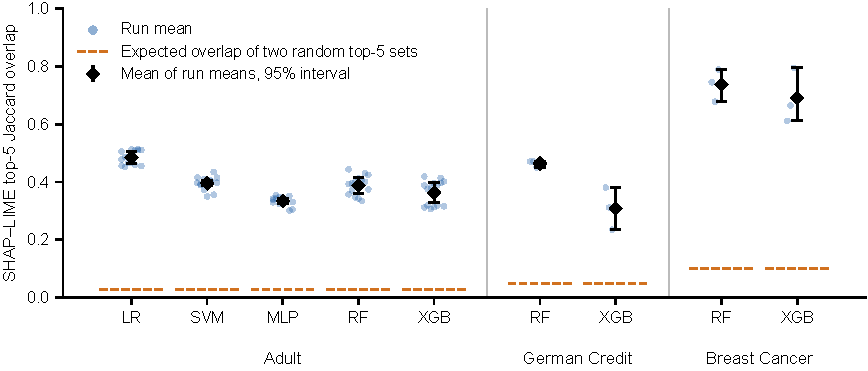
\includegraphics[width=\textwidth]{figures/fig1_top5_overlap.pdf}
\caption{Top-5 overlap between SHAP and LIME by dataset and model family. Each point is the mean of one run}
\label{fig:overlap}
\end{figure*}

\subsection{Model Family, Sampling Intensity and Dataset (RQ2)}

On Adult, agreement differed between model families. The overlap was highest for
logistic regression (<<agree|exp2_adult|logreg|top5_jaccard|est>>) and lowest for the
multilayer perceptron (<<agree|exp2_adult|mlp|top5_jaccard|est>>); the intervals of
these two families do not overlap. Rank concordance was close to zero for the
multilayer perceptron (<<agree|exp2_adult|mlp|kendall_tau_b|est>>) and for gradient
boosting (<<agree|exp2_adult|xgb|kendall_tau_b|est>>, with an interval that includes
zero). On German Credit the overlap was higher for the random forest
(<<agree|german_credit|rf|top5_jaccard|est>>) than for gradient boosting
(<<agree|german_credit|xgb|top5_jaccard|est>>); on Breast Cancer the two families were
close.

The sampling intensity had no visible effect: pooled over models, the top-5 overlap on
Adult was <<int|n_50|top5_jaccard|est>>, <<int|n_100|top5_jaccard|est>> and
<<int|n_200|top5_jaccard|est>> for 50, 100 and 200 instances per quadrant. Explaining
more instances makes the estimate of agreement more precise; it does not change the
agreement.

The dataset mattered most. Adult and German Credit, with many one-hot encoded features,
gave similar and low agreement; Breast Cancer, with 30 numeric features, gave much
higher agreement for the same two model families. Three datasets do not allow this
difference to be attributed to a specific property of the data.

\subsection{Agreement of Signs (Post Hoc)}
\label{sec:results:sign}

The planned sign agreement on shared top-5 features was
<<agree|exp2_adult|all|sign_agreement|est>> on Adult,
<<agree|german_credit|all|sign_agreement|est>> on German Credit and
<<agree|breast_cancer|all|sign_agreement|est>> on Breast Cancer. The last value is below
one half, on the dataset where the two methods agree most on which features matter. This
led to the post hoc analysis in Table~\ref{tab:sign} and Fig.~\ref{fig:sign}.

Sign agreement depended strongly on the predicted class. On Breast Cancer it was
<<sign|breast_cancer|all|0|est>> for instances predicted as class~0 and
<<sign|breast_cancer|all|1|est>> for instances predicted as class~1. On Adult it was
<<sign|exp2_adult|all|1|est>> for class~1 and <<sign|exp2_adult|all|0|est>> for
class~0, and the same pattern appeared in four of the five model families; the
multilayer perceptron was the exception.

The reason is that the two methods return different quantities
(Section~\ref{sec:methods:explainers}). The LIME coefficient of a continuous feature is a
local slope. The slope of a feature with a monotone effect has the same sign for most
instances. A SHAP value is a contribution relative to the expected output: for the same
feature it is positive for instances on one side of the reference and negative on the
other. The two signs therefore coincide for the instances of one predicted class and
differ for the other. The constancy measure confirms it: on Breast Cancer, a feature
kept its majority sign in <<const|breast_cancer|all|lime|est>> of its LIME explanations
and in <<const|breast_cancer|all|shap|est>> of its SHAP explanations
(<<const|german_credit|all|lime|est>> and <<const|german_credit|all|shap|est>> on German
Credit; <<const|exp2_adult|all|lime|est>> and <<const|exp2_adult|all|shap|est>> on
Adult, where most features are one-hot indicators).

Sign agreement between SHAP and LIME without discretisation is thus not a measure of
disagreement about the direction of an effect. It measures mostly on which side of the
reference the instance lies.

\begin{table}[t]
\renewcommand{\arraystretch}{\tablestretch}
\centering
\caption{Sign agreement on shared top-5 features, overall and by predicted class, and constancy of the sign of a feature across instances (share of instances with the majority sign). Post hoc}
\label{tab:sign}
\footnotesize
\setlength{\tabcolsep}{\tightcolsep}
\begin{tabular}{llrrrrr}
\hline
 & & \multicolumn{3}{c}{Sign agreement} & \multicolumn{2}{c}{Constancy} \\
Dataset & Model & All & Cl.~0 & Cl.~1 & SHAP & LIME \\
\hline
% GENERATED by scripts/build_paper_e.py -- do not edit
Adult & LR & 0.696 & 0.527 & 0.864 & 0.947 & 0.947 & 0.948 \\
 & SVM & 0.829 & 0.332 & 0.956 & 0.952 & 0.918 & 0.960 \\
 & MLP & 0.689 & 0.706 & 0.672 & 0.951 & 0.940 & 0.962 \\
 & RF & 0.696 & 0.418 & 0.975 & 0.948 & 0.913 & 0.984 \\
 & XGB & 0.682 & 0.443 & 0.916 & 0.925 & 0.911 & 0.939 \\
 & All & 0.717 & 0.506 & 0.875 & 0.945 & 0.927 & 0.958 \\
\hline
German Credit & RF & 0.470 & 0.608 & 0.430 & 0.985 & 0.990 & 0.983 \\
 & XGB & 0.553 & 0.716 & 0.494 & 0.934 & 0.933 & 0.934 \\
 & All & 0.511 & 0.662 & 0.462 & 0.960 & 0.962 & 0.959 \\
\hline
Breast Cancer & RF & 0.377 & 0.975 & 0.041 & 0.997 & 1.000 & 0.995 \\
 & XGB & 0.371 & 0.979 & 0.032 & 0.983 & 0.983 & 0.983 \\
 & All & 0.374 & 0.977 & 0.036 & 0.990 & 0.991 & 0.989 \\
\hline

\end{tabular}
\end{table}

\begin{figure*}[t]
\centering
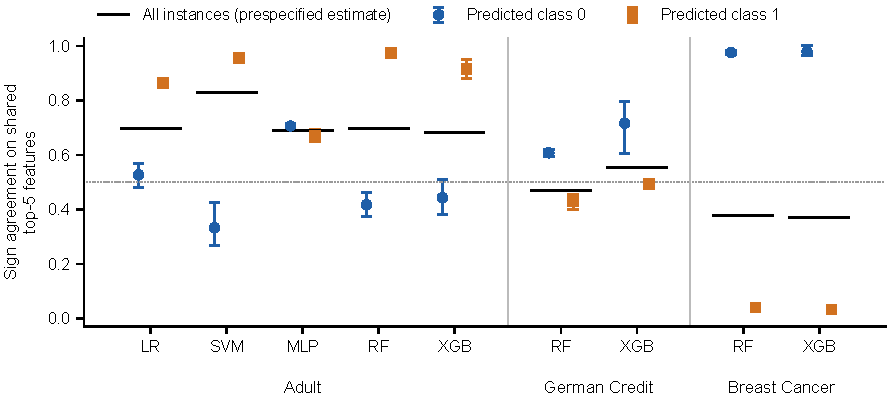
\includegraphics[width=\textwidth]{figures/fig2_sign_by_class.pdf}
\caption{Sign agreement between SHAP and LIME by predicted class, with seed-clustered 95\% intervals. The dotted line marks one half}
\label{fig:sign}
\end{figure*}

\subsection{Correct and Misclassified Instances (RQ3)}

Table~\ref{tab:correctness} and Fig.~\ref{fig:correctness} give the difference in top-5
overlap between misclassified and correctly classified instances. The direction was not
consistent. For the multilayer perceptron, agreement was lower on misclassified
instances (difference <<corr|exp2_adult|mlp|diff>>, interval
<<corr|exp2_adult|mlp|lo>> to <<corr|exp2_adult|mlp|hi>>, same direction in all five
seeds). For the random forest it was higher (<<corr|exp2_adult|rf|diff>>,
<<corr|exp2_adult|rf|lo>> to <<corr|exp2_adult|rf|hi>>, all five seeds), and slightly
higher for gradient boosting (<<corr|exp2_adult|xgb|diff>>). For logistic regression and
the support vector machine the difference was near zero. On German Credit the
differences were small and negative, with three seeds. On Breast Cancer no run had ten
misclassified instances, so the contrast could not be estimated. The largest difference in absolute value was that of the
multilayer perceptron, small compared with the differences between model families.

\begin{table}[t]
\renewcommand{\arraystretch}{\tablestretch}
\centering
\caption{Top-5 overlap for correctly classified (C) and misclassified (M) instances. Diff.\ is M minus C; Neg.\ is the number of seeds with a negative difference; GC is German Credit}
\label{tab:correctness}
\footnotesize
\setlength{\tabcolsep}{\tightcolsep}
\begin{tabular}{llrrrlr}
\hline
Data & Model & C & M & Diff. & 95\% interval & Neg. \\
\hline
% GENERATED by scripts/build_paper_e.py -- do not edit
Adult & LR & 0.486 & 0.483 & $-$0.003 & [$-$0.023, 0.012] & 2/5 \\
Adult & SVM & 0.388 & 0.387 & $-$0.001 & [$-$0.017, 0.020] & 3/4 \\
Adult & MLP & 0.364 & 0.305 & $-$0.059 & [$-$0.069, $-$0.049] & 5/5 \\
Adult & RF & 0.367 & 0.412 & 0.045 & [0.029, 0.064] & 0/5 \\
Adult & XGB & 0.356 & 0.370 & 0.014 & [0.003, 0.022] & 1/5 \\
GC & RF & 0.469 & 0.452 & $-$0.017 & [$-$0.036, 0.001] & 2/3 \\
GC & XGB & 0.311 & 0.305 & $-$0.005 & [$-$0.010, $-$0.001] & 3/3 \\
\hline

\end{tabular}
\end{table}

\begin{figure}[t]
\centering
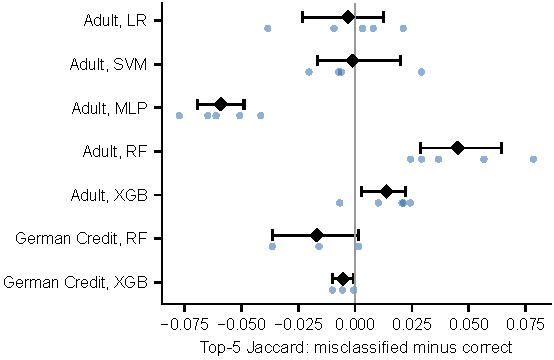
\includegraphics[width=\columnwidth]{figures/fig3_correctness.pdf}
\caption{Difference in top-5 overlap, misclassified minus correct. Points are seeds; diamonds are means with seed-clustered 95\% intervals}
\label{fig:correctness}
\end{figure}

\subsection{Disagreement and Explanation Quality (RQ4)}

Table~\ref{tab:quality} and Fig.~\ref{fig:quality} give the within-run Spearman
correlation between disagreement and the four quality values. The clearest pattern
concerns the fidelity of LIME: on Adult the correlation was negative for all five model
families (from <<qrange|exp2_adult|lime_fidelity|min>> to
<<qrange|exp2_adult|lime_fidelity|max>>), and it was negative on German Credit
(<<qrange|german_credit|lime_fidelity|min>> and
<<qrange|german_credit|lime_fidelity|max>>). The two methods disagreed more on the
instances where the local linear model of LIME reproduced the model less well. The
correlations with the fidelity of SHAP were closer to zero and of mixed sign.

For stability there was no common pattern. On Adult the correlations were small and
mostly positive, except for the multilayer perceptron. On Breast Cancer with the random
forest, disagreement was higher for instances with less stable explanations of either
method (<<qual|breast_cancer|rf|shap_stability>> and
<<qual|breast_cancer|rf|lime_stability>>), with three runs. These are associations within
runs; they do not show that low fidelity causes disagreement.

\begin{table}[t]
\renewcommand{\arraystretch}{\tablestretch}
\centering
\caption{Mean within-run Spearman correlation between disagreement ($1 - J_5$) and explanation quality. Fid.: fidelity; Stab.: stability}
\label{tab:quality}
\small
\setlength{\tabcolsep}{\mediumcolsep}
\begin{tabular}{llrrrr}
\hline
 & & \multicolumn{2}{c}{SHAP} & \multicolumn{2}{c}{LIME} \\
Dataset & Model & Fid. & Stab. & Fid. & Stab. \\
\hline
% GENERATED by scripts/build_paper_e.py -- do not edit
Adult & LR & $-$0.01 & 0.09 & $-$0.40 & 0.12 \\
 & SVM & $-$0.05 & 0.06 & $-$0.45 & 0.12 \\
 & MLP & $-$0.06 & $-$0.24 & $-$0.19 & $-$0.07 \\
 & RF & $-$0.22 & 0.23 & $-$0.27 & 0.10 \\
 & XGB & $-$0.15 & 0.14 & $-$0.40 & 0.11 \\
\hline
German Credit & RF & $-$0.05 & $-$0.06 & $-$0.26 & $-$0.10 \\
 & XGB & $-$0.04 & 0.02 & $-$0.24 & $-$0.15 \\
\hline
Breast Cancer & RF & $-$0.06 & $-$0.56 & $-$0.28 & $-$0.54 \\
 & XGB & 0.22 & $-$0.34 & 0.01 & $-$0.27 \\
\hline

\end{tabular}
\end{table}

\begin{figure*}[t]
\centering
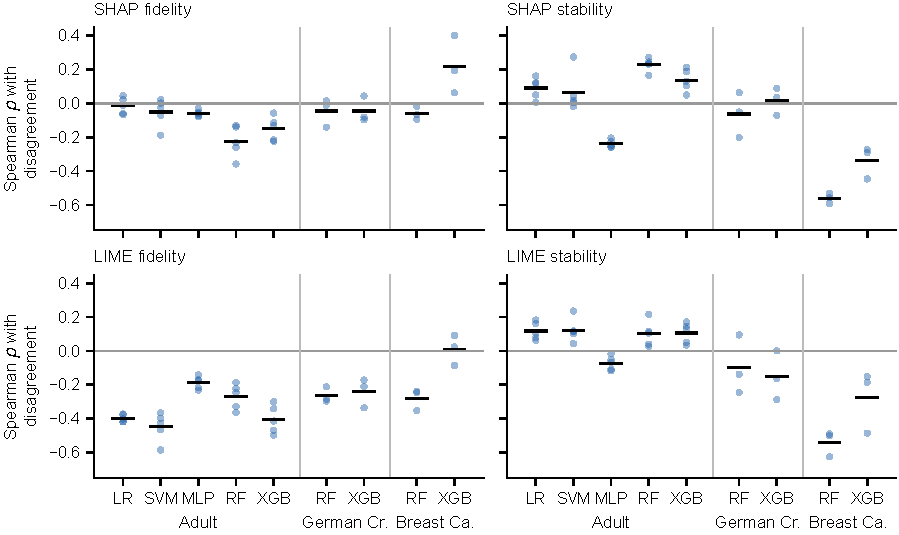
\includegraphics[width=\textwidth]{figures/fig4_quality.pdf}
\caption{Within-run Spearman correlation between disagreement and four quality values. Points are seeds; bars are means over seeds}
\label{fig:quality}
\end{figure*}

\subsection{Feature Sets of Anchors and DiCE (Secondary)}

Table~\ref{tab:secondary} gives the overlap between feature sets on Adult. The features
in an Anchors rule overlapped more with the SHAP top-5 set
(<<sec|shap_anchors|all|est>>) than with the LIME top-5 set
(<<sec|lime_anchors|all|est>>). The features changed by DiCE overlapped little with any
other set (at most <<sec|lime_dice|all|est>>). These methods answer different questions,
a sufficient condition and a minimal change, so a low overlap is not an error of either
method; it shows that their features cannot be substituted for those of an attribution
method.

\begin{table}[t]
\renewcommand{\arraystretch}{\tablestretch}
\centering
\caption{Jaccard overlap between feature sets on Adult (SHAP, LIME: top-5 features; Anchors: rule features; DiCE: changed features): mean of run means and seed-clustered 95\% interval}
\label{tab:secondary}
\footnotesize
\setlength{\tabcolsep}{\tightcolsep}
\begin{tabular}{lrrrl}
\hline
Feature sets & Runs & Pairs & Mean & 95\% int. \\
\hline
% GENERATED by scripts/build_paper_e.py -- do not edit
SHAP vs. Anchors & 56 & 14,584 & 0.348 & [0.340, 0.356] \\
LIME vs. Anchors & 57 & 19,095 & 0.240 & [0.234, 0.247] \\
SHAP vs. DiCE & 67 & 25,248 & 0.078 & [0.068, 0.087] \\
LIME vs. DiCE & 68 & 29,830 & 0.078 & [0.074, 0.085] \\
Anchors vs. DiCE & 53 & 18,578 & 0.068 & [0.062, 0.075] \\
\hline

\end{tabular}
\end{table}

\section{Discussion}
\label{sec:discussion}

\textbf{The choice of explainer changes the explanation.} On two of the three datasets,
SHAP and LIME shared on average fewer than three of their five most important features,
and the order of the features was almost unrelated for two model families. A user who
reads a top-5 list would see a different list with the other method. This agrees with
the disagreement reported by Krishna et al. \cite{krishna2024disagreement} and extends
it with the run as the unit of analysis: the result is stable across five seeds and three
sampling intensities, so it is not an artefact of a particular sample of instances.

\textbf{Agreement is a property of the model and the data.} The differences between
model families and between datasets were larger than every other effect measured here.
This is consistent with the view that the methods approximate the model in different
neighbourhoods \cite{han2022which}: where the model is close to linear around the
instance, as for logistic regression, the approximations coincide more. The high
agreement on Breast Cancer indicates that low agreement is not inevitable. A report of
explainer agreement should therefore state the model family and the dataset, and should
not be generalised from one of them.

\textbf{Signs need the same quantity.} The sign analysis shows a risk for any study that
compares the direction of attributions between methods. A LIME coefficient without
discretisation is a slope; a SHAP value is a contribution relative to a reference
\cite{garreau2020explaining,lundberg2017unified}. Their signs can differ for every
instance of one class while the two methods describe the same relation between the
feature and the output. Before signs are compared, the two explanations should be
brought to the same quantity, for example by multiplying the slope by the deviation of
the feature from the reference, or by using LIME with discretisation, whose weights refer
to the value of the instance. The measures of overlap and rank used for RQ1 to RQ4 depend
on absolute values and are not affected by this difference of sign, although a slope and
a contribution also differ in magnitude, which is one source of the low rank
concordance.

\textbf{Disagreement and correctness.} Agreement was not consistently lower when the
model was wrong. The direction depended on the model family and the differences were
small. Disagreement between explainers is therefore not a usable signal of a wrong
prediction in these data.

\textbf{Disagreement and LIME fidelity.} Disagreement was higher where LIME fitted the
model less well. Part of the disagreement may thus come from the approximation error of
the local linear model, not from two valid but different views of the model. The
fidelity of LIME, which is available at no extra cost, can indicate the instances for
which the two methods are more likely to differ.

\textbf{Limitations.} The study covers three tabular binary datasets and one
configuration of each explainer; other kernel widths, sample sizes or discretisation
settings of LIME may change the estimates. There are five seeds on Adult and three on
the other datasets, so the intervals are imprecise and the analyses of RQ2 to RQ4 are
exploratory. Only the ten largest features of each explanation were stored, which limits
the rank measure to that list. One-hot columns were treated as separate features; an
analysis by original variable would give higher overlap. TreeSHAP was used with its
default output, which for gradient boosting is the log-odds and for the random forest
the probability, while LIME explains the probability; this affects magnitudes and ranks,
not signs. KernelSHAP failed for part of the SVM instances, so that family has fewer
pairs. The models of the two smaller datasets were regenerated from the training recipe
and validated against stored metrics and predictions, not compared byte by byte with the
original binaries. For the Adult random forest, the stored binary does not reproduce all
the predictions recorded in the runs; the analysis uses only the recorded outputs, and
the paired SHAP and LIME records agree on every label and prediction. The sign analysis
is post hoc.

\section{Conclusions and Future Work}
\label{sec:conclusions}

For the same instance and model, SHAP and LIME agreed only partly on the most important
features: the mean top-5 overlap was <<agree|exp2_adult|all|top5_jaccard|est>> on Adult,
<<agree|german_credit|all|top5_jaccard|est>> on German Credit and
<<agree|breast_cancer|all|top5_jaccard|est>> on Breast Cancer. Agreement depended on the model family and the dataset, not on the number
of explained instances, and it was not consistently lower for misclassified instances.
Disagreement was associated with a lower local fidelity of LIME. The sign agreement
between SHAP and LIME without discretisation followed the predicted class, because one
method returns slopes and the other contributions; it should not be used as a measure of
disagreement unless both explanations are first expressed as the same quantity.

Two practical consequences follow. An explanation shown to a user should name the
explainer, since another explainer would often show other features. And a comparison of
explainers should check, before any measure is computed, what each stored value means.

Future work will convert LIME coefficients into contributions to measure sign agreement
on a common quantity, repeat the analysis by original variable, vary the LIME
configuration, and add datasets to separate the effect of the number and type of
features from that of the model family.

\section*{Data Availability}
\iffull
The three datasets are public
\cite{becker1996adult,hofmann1994statlog,wolberg1993breast}. The code, the per-instance
run outputs, the new LIME cohort, the registered analysis plan and every result file are
available at \url{https://github.com/jonnabio/xai-eval-framework} (release
\texttt{\papererelease}), archived at \paperearchive. Every number, table
and figure in this article is generated from those files by the scripts described in
\texttt{docs/reports/paper\_e/README.md}.
\else
The three datasets are public
\cite{becker1996adult,hofmann1994statlog,wolberg1993breast}. The code, the per-instance
run outputs, the new LIME cohort, the registered analysis plan and every result file are
in a public repository, with scripts that generate every number, table and figure in
this article; its address is withheld for blind review.
\fi

{
\bibliographystyle{cys}
\bibliography{references}
}

% Journal footer, as in the CyS template (example.tex). The journal fills in the dates,
% which it prints day first (its example reads "accepted on 16/01/2017").
{\vskip 12pt}
\noindent
\footnotesize {\textit{Article received on DD/MM/YYYY; accepted on DD/MM/YYYY.\iffull\\
{*}Corresponding author is Jonathan Herrera-V\'asquez.\fi}}

\end{document}
